\documentclass[landscape,a0paper,fontscale=0.285,table]{baposter} % Adjust the font scale/size here

\usepackage{graphicx} % Required for including images
\usepackage{amsmath} % For typesetting math
\usepackage{amssymb} % Adds new symbols to be used in math mode
\usepackage{natbib}
\setlength{\bibsep}{0.0pt}
\usepackage{enumitem} % Used to reduce itemize/enumerate spacing
\usepackage{palatino} % Use the Palatino font
\usepackage[font=small,labelfont=bf]{caption} % Required for specifying captions to tables and figures
\usepackage{multicol} % Required for multiple columns
\setlength{\columnsep}{1.5em} % Slightly increase the space between columns
\setlength{\columnseprule}{0mm} % No horizontal rule between columns

\usepackage{diagbox}
\usepackage{multirow}
\usepackage{booktabs}

\newcommand{\compresslist}{ % Define a command to reduce spacing within itemize/enumerate environments, this is used right after \begin{itemize} or \begin{enumerate}
\setlength{\itemsep}{1pt}
\setlength{\parskip}{0pt}
\setlength{\parsep}{0pt}
}

\newcommand{\subcaption}[1]% %1 = text
{\par\vskip\abovecaptionskip
\centerline{#1}%
\vskip\belowcaptionskip\par}

% create subfigure environment
\def\subfigure{\let\oldcaption=\caption
\let\caption=\subcaption
\minipage}
\def\endsubfigure{\endminipage
\let\caption=\oldcaption}


\definecolor{lightred}{rgb}{0.74117,0.12549,0.1921} % Defines the color used for content box headers

\begin{document}

\begin{poster}
{
headerborder=closed, % Adds a border around the header of content boxes
colspacing=1em, % Column spacing
bgColorOne=white, % Background color for the gradient on the left side of the poster
bgColorTwo=white, % Background color for the gradient on the right side of the poster
borderColor=lightred, % Border color
headerColorOne=lightred, % Background color for the header in the content boxes (left side)
headerColorTwo=lightred, % Background color for the header in the content boxes (right side)
headerFontColor=white, % Text color for the header text in the content boxes
boxColorOne=white, % Background color of the content boxes
textborder=roundedleft, % Format of the border around content boxes, can be: none, bars, coils, triangles, rectangle, rounded, roundedsmall, roundedright or faded
eyecatcher=true, % Set to false for ignoring the left logo in the title and move the title left
headerheight=0.1\textheight, % Height of the header
headershape=roundedright, % Specify the rounded corner in the content box headers, can be: rectangle, small-rounded, roundedright, roundedleft or rounded
headerfont=\Large\bf\textsc, % Large, bold and sans serif font in the headers of content boxes
%textfont={\setlength{\parindent}{1.5em}}, % Uncomment for paragraph indentation
linewidth=2pt % Width of the border lines around content boxes
}
%----------------------------------------------------------------------------------------
%	TITLE SECTION 
%----------------------------------------------------------------------------------------
%
{
\includegraphics[height=4em]{imgs/logo1.png}} % First university/lab logo on the left
{\bf\textsc{Hybrid Distributional and Definitional Word Vectors}\vspace{0.05em}} % Poster title
{Haiyuan Mei and Ranjani Iyer\\
Stanford University, Department of Computer Science} % Author names and istitution(s)
{
\includegraphics[height=4em]{imgs/logo2.jpg}} % Second university/lab logo on the right

%----------------------------------------------------------------------------------------
%	Overview
%----------------------------------------------------------------------------------------

\headerbox{Overview}{name=overview,column=0,span=2,row=0}{

\begin{itemize}[leftmargin=*]
\item \textbf{Motivation}: OOV problem, and exploration of word definitions in downstream NLP tasks.
\item \textbf{Prior methods:} Def2Vec, on-the-fly embeddings capable of capturing OOV words and limited usage exploration.\cite{luong_2013}
\item \textbf{Approach: HybridVec}  Generate word embedding from word definitions, combine it with distributed representations and explore the possibility or improving downstream NLP tasks.
\item \textbf{Evaluation:} Intrinsic word embedding benchmarks and Extrinsic NMT evaluation, shown to improve translation perplexities and capture complementary aspect of word regarding distributed representation.
\end{itemize} 

\begin{center}
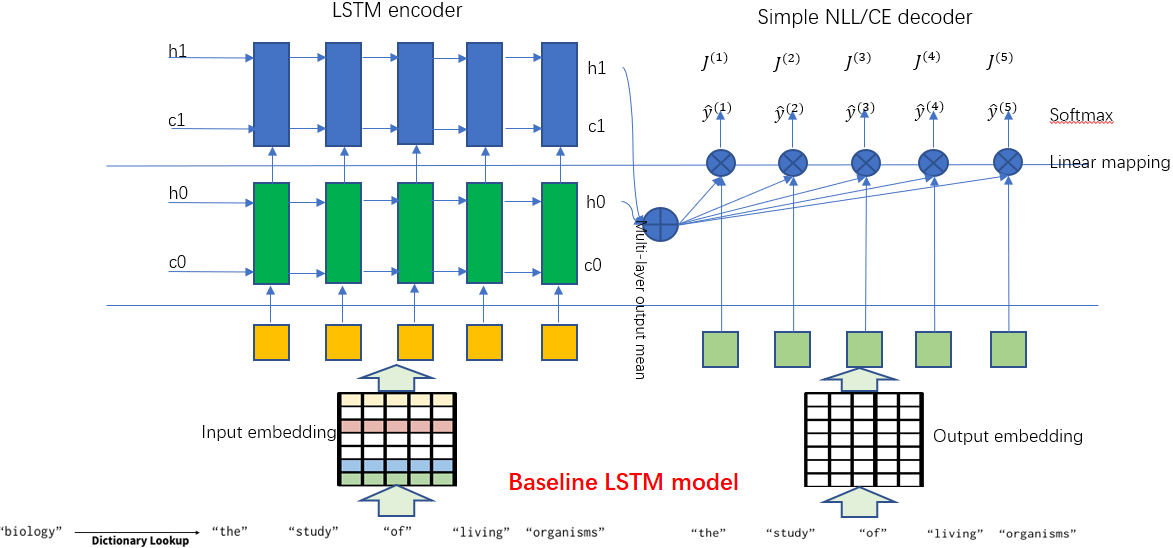
\includegraphics[width=0.9\linewidth]{imgs/lstmnll}
\end{center}

}

%----------------------------------------------------------------------------------------
%	Results
%----------------------------------------------------------------------------------------

\headerbox{Results}{name=results,column=2,span=2,row=0}{

\begin{itemize}
\item Word embeddings benchmarks for GloVe, LSTM Baseline and Seq2seq model. From the result it is obvious that LSTM baseline model is roughly at the level of distributional method; s2s model on the other hand shows very limited evidence of such capability.  (https://github.com/kudkudak/word-embeddings-benchmarks):
\end{itemize}
\begin{center}
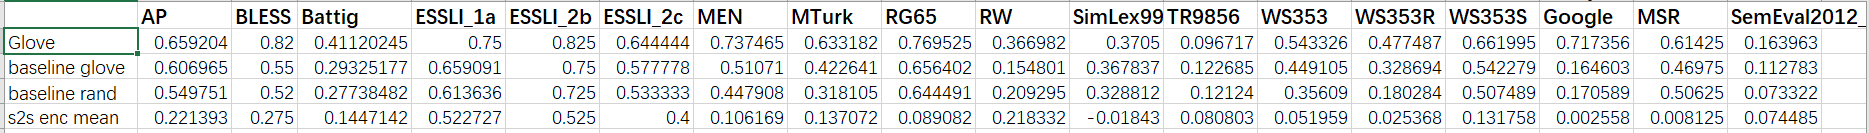
\includegraphics[width=\linewidth]{imgs/intrinsic}
\end{center}
\begin{itemize}
\begin{itemize}
\compresslist
\item GloVe: WEB benchmark for GloVe vectors
\item Baseline glove: WEB benchmark for LSTM baseline model initialized from GloVe embeddings
\item Baseline rand: WEB benchmark for LSTM baseline model initialized randomly
\item s2s enc mean: WEB benchmark for Seq2seq model with encoder output mean as the def vec.
\end{itemize}

\item Standard NMT metrics compare performance improvement using LSTM baseline vector and GloVe:
\end{itemize}
	
\begin{center}
\label{my-label}
\begin{tabular}{@{}c|c|cccccc@{}}
                     Vocab        & 400k  & \textbf{10k  +   Glove}  & 10k  + Baseline & 10k \\ \hline
\multicolumn{1}{l|}{Perplexities} & 38.15 & - & - &  41.82  \\
\multicolumn{1}{l|}{BLEU}         & 5.55  & - & - &  4.44    
\end{tabular}
\end{center}

}


%----------------------------------------------------------------------------------------
%	Analysis
%----------------------------------------------------------------------------------------

\headerbox{Analysis}{name=analysis,below=results,column=2,span=2,row=1}{

\begin{center}

\end{center}

\vspace*{-0.7cm}
\begin{itemize}
\compresslist
\item LSTM baseline vectors tend to cluster more closely in feature space. Need to train from a broader data source.
\item Glove vectors make use of feature space more efficiently, capable of grasping more sutle meaning of words.
\end{itemize}
\vspace*{-0.2cm}
 \begin{subfigure}{0.54\textwidth}
  \centering
  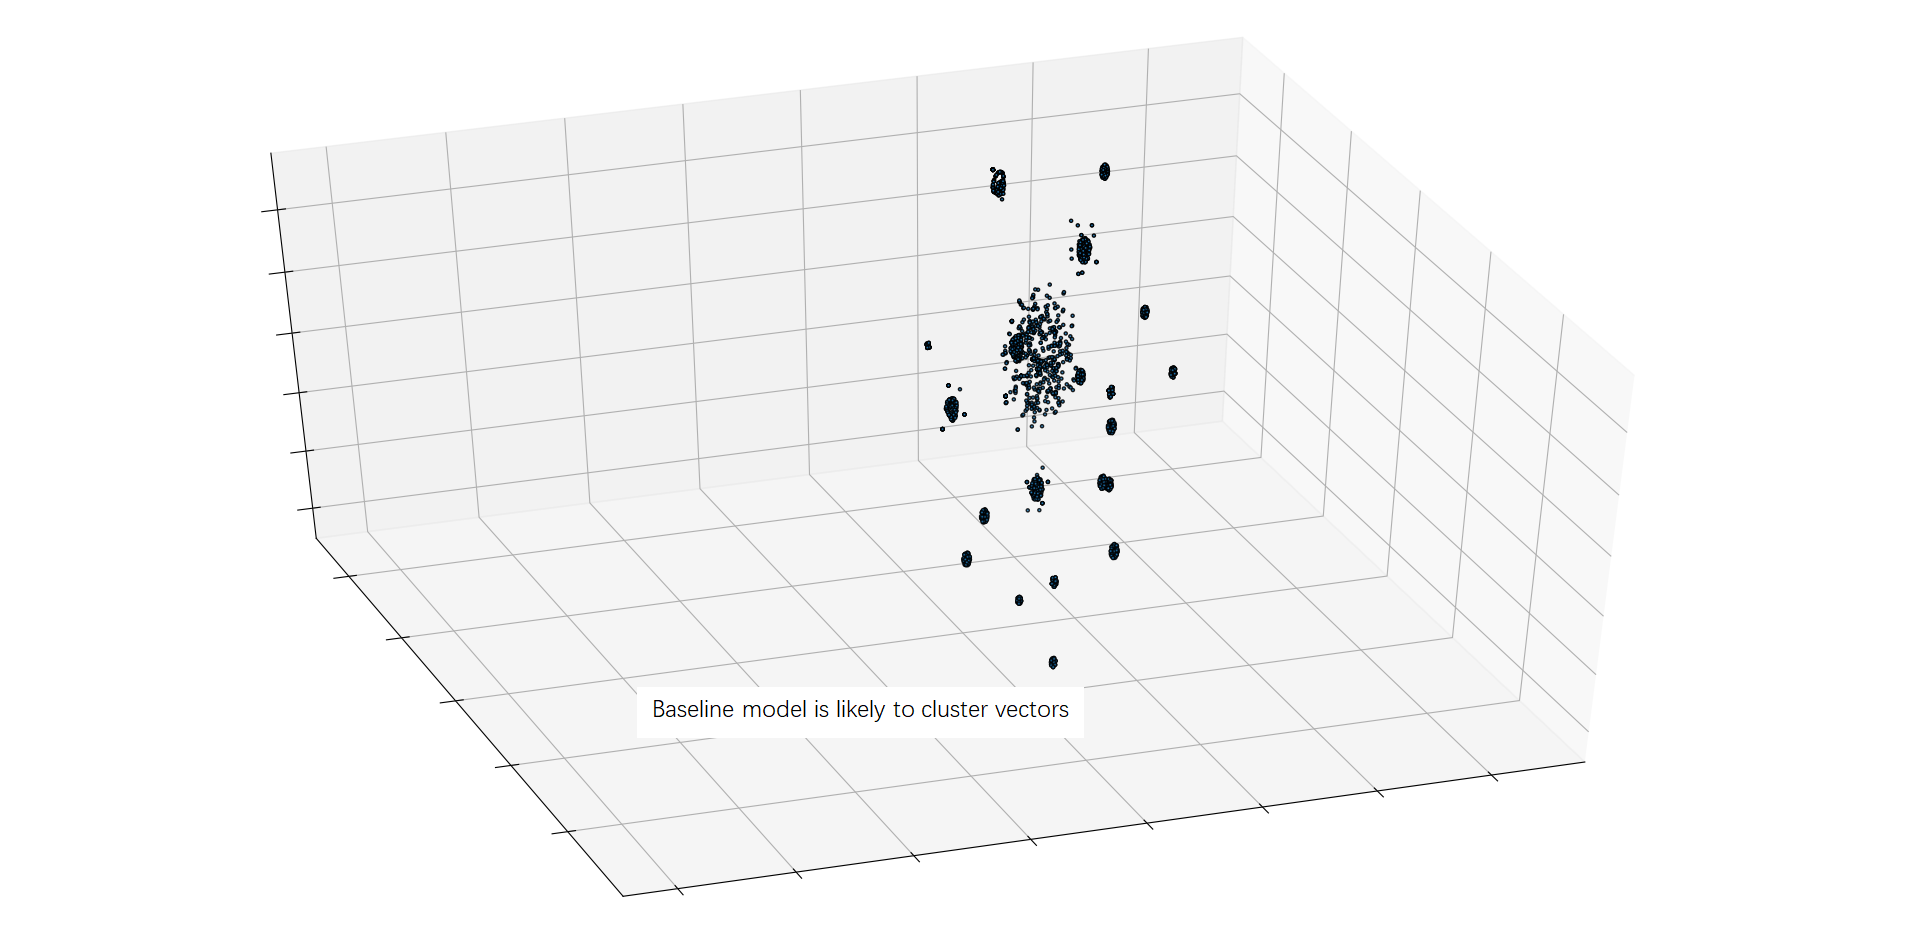
\includegraphics[width=0.9\textwidth]{imgs/lstmbaseline-tsne.png}
  \vspace*{-0.1cm}
  \subcaption{3D tSNE: LSTM Baseline vectors is likely to cluster}
 \end{subfigure}
  \begin{subfigure}{0.41\textwidth}
  \vspace*{0.1cm}
  \centering
  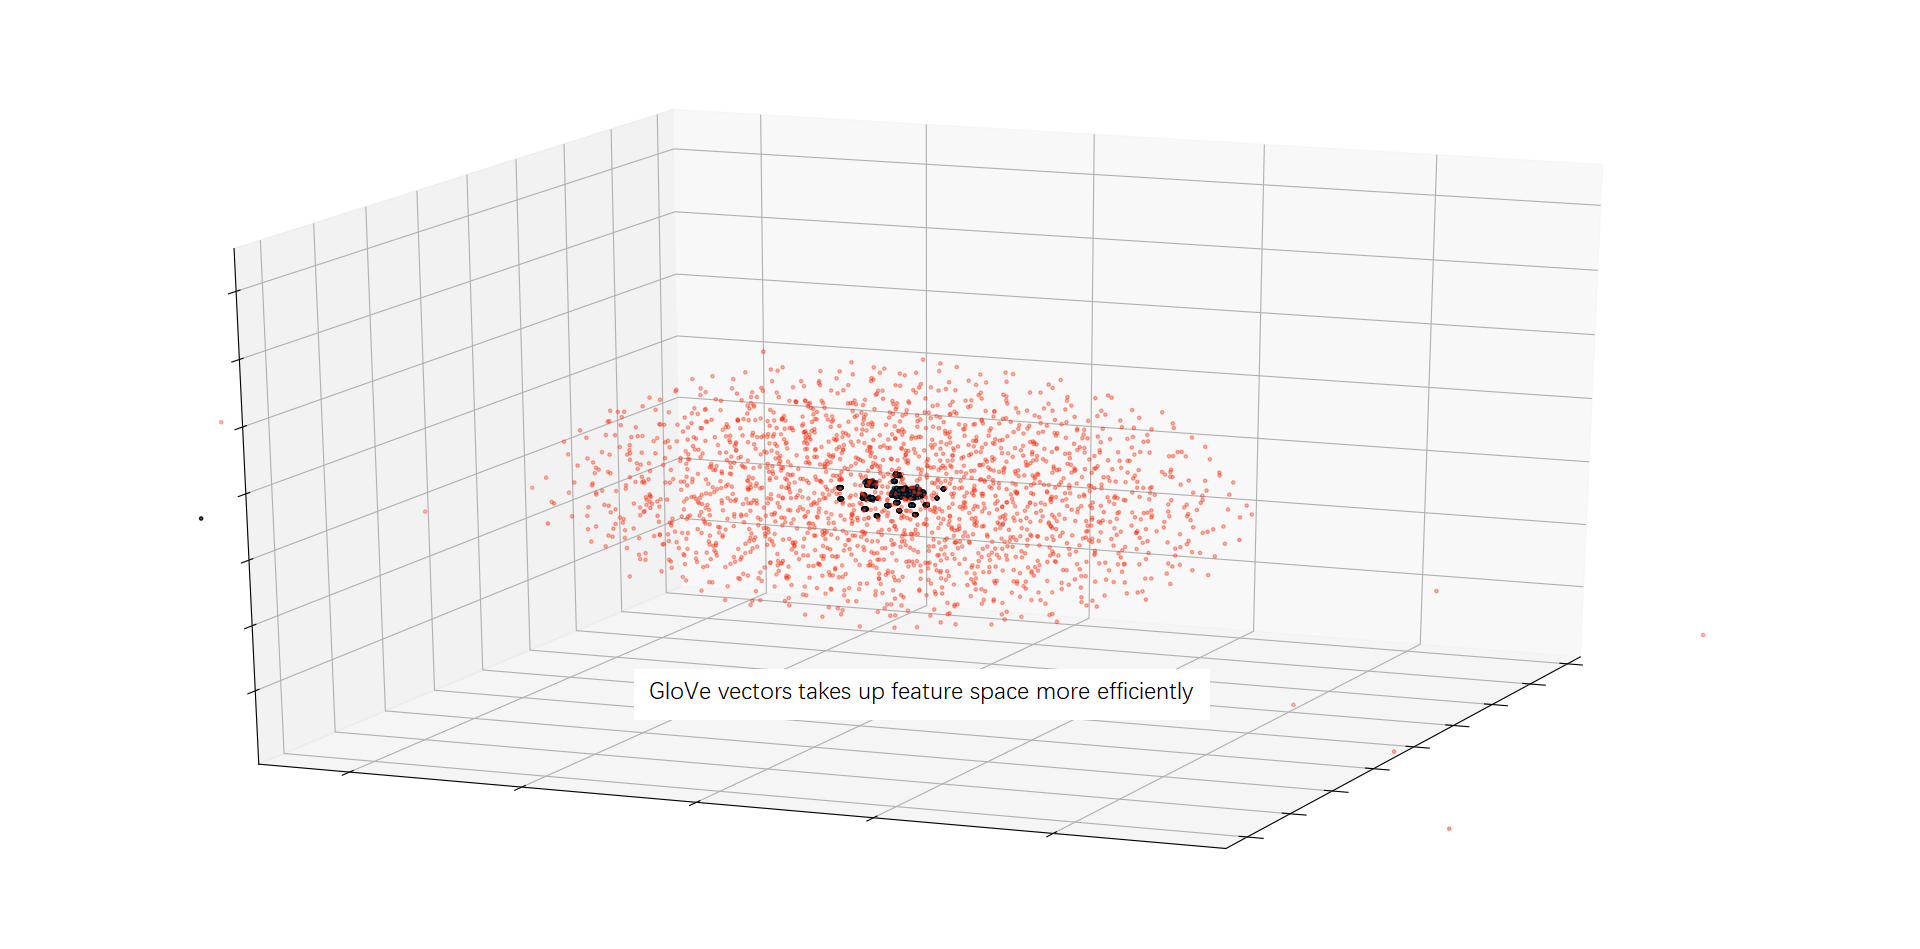
\includegraphics[width=0.9\textwidth]{imgs/lstmglove.png}
  \vspace*{0.14cm}

  \subcaption{tSNE for both: GloVe uses feature space more efficiently}
 \end{subfigure}\hfil

}

%----------------------------------------------------------------------------------------
%	Discussion
%----------------------------------------------------------------------------------------

\headerbox{Discussion}{name=conclusion,column=2,row=2,below=analysis}{

\begin{itemize}[leftmargin=*]
\compresslist
\item Additional plans for model: greater regularization, inputting multiple definitions, inputting sentence structure, try other embeddings. 
\item Plan to open source pretrained model and create demo with reverse-dict.xyz
\end{itemize}

}

%----------------------------------------------------------------------------------------
%	REFERENCES
%----------------------------------------------------------------------------------------

\headerbox{References}{name=references,column=3, row=2, below=analysis, bottomaligned=conclusion}{

\renewcommand{\section}[2]{\vskip 0.05em} % Get rid of the default "References" section title
\tiny{ % Reduce the font size in this block
\bibliographystyle{unsrt}
\bibliography{refs}
}
}

%----------------------------------------------------------------------------------------
%	MODEL
%----------------------------------------------------------------------------------------

\headerbox{Model}{name=details,column=0,below=overview,bottomaligned=conclusion}{

\begin{itemize}[leftmargin=*]
\item \textbf{Baseline LSTM:} A two-layer LSTM encoder, Simple linear decoder and NLL loss. Encoder layer hidden output  denotes the final definition word vector.

\item \textbf{Seq2seq:} A two-layer LSTM encoder with dropouts plus a two layer LSTM decoder with attention.

\item Input is given as sequence of padded pretrained word vectors

\item The NMT model is a classic Seq2Seq with attention taken directly from \textbf{OpenNMT} \cite{2017opennmt}:\\


\end{itemize}


}

%----------------------------------------------------------------------------------------
%	TRAINING
%----------------------------------------------------------------------------------------

\headerbox{Training}{name=training,column=1,below=overview,bottomaligned=conclusion}{

\begin{itemize}[leftmargin=*]

\item \textbf{Dataset: GloVe} \cite{pennington_2014}. All models are trained on pretrained 300d GloVe vectors based on a crawl of 2014 Wikipedia. \\
Definitions retrieved from \textbf{WordNet}\cite{miller_1995}.

\item \textbf{HybridVec Implementation:} Pytorch, Adam optimizer, Xavier initialization, hidden size 150, learning rate of {1e-4}, batch size  64, 15/20 epochs. 

\item \textbf{Intrinsic evaluation:} Word embedding benchmarks (https://github.com/kudkudak/word-embeddings-benchmarks).

\item \textbf{NMT Dataset:} OpenNMT-py demo(10k) dataset. Only for comparasion between GloVe and HybridVec.

\end{itemize}


}




\end{poster}

\end{document}